
\subsection{Compositional audit of the confound}\label{sec:compaudit}
What separates the classes if not labels? Study 18 computes first-order
composition for the three label $\times$ review-status groups of the large
dataset (Table~\ref{tab:compaudit}, Figure~\ref{fig:composition}).

\begin{table}[h]\centering\small
\caption{Composition by label and review status over all 49{,}256 large
dataset records (train+val+test). Charge is the integer formal-charge
proxy of Appendix~\ref{app:encoding}.}
\label{tab:compaudit}
\begin{tabular}{lrcccc}
\hline
Group & $n$ & Length & KD hydropathy & Net charge & Aromatic \% \\
\hline
pos reviewed & 2,886 & 66.2$\pm$36.5 & +0.03$\pm$0.59 & +2.39$\pm$4.41 & 7.9 \\
pos unreviewed & 21,742 & 96.7$\pm$30.7 & -0.06$\pm$0.33 & +2.93$\pm$4.75 & 8.7 \\
neg reviewed & 24,628 & 93.2$\pm$32.8 & -0.29$\pm$0.58 & +3.16$\pm$8.12 & 7.3 \\
\hline
\end{tabular}
\end{table}

\begin{figure}[h]\centering
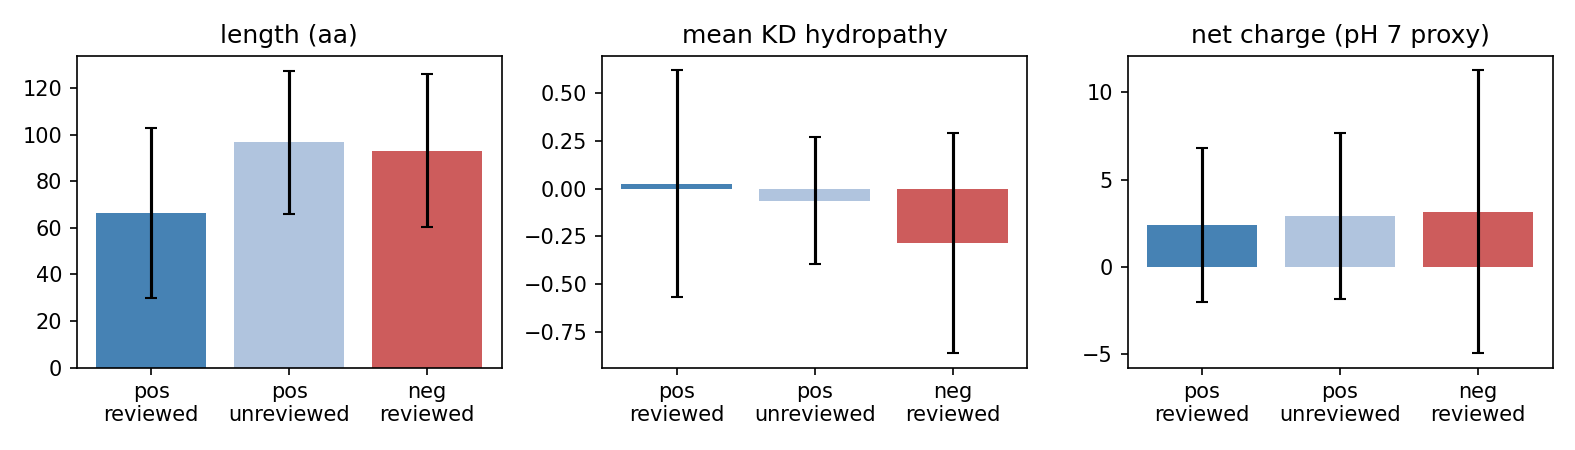
\includegraphics[width=\textwidth]{fig_composition.png}
\caption{Length, hydropathy and charge by group (bars: mean $\pm$ sd).}
\label{fig:composition}
\end{figure}

The result is a caution against a simple story. First-order composition
barely separates the groups: mean charge spans only $+2.4$ to $+3.2$, mean
hydropathy $-0.29$ to $+0.03$. The one large gap is length: reviewed
positives average 66 aa against 93--97 aa for both other groups, a
curation artifact (reviewed AMP records skew to mature short peptides,
unreviewed records to longer precursors). Length is trivially learnable by
a CNN through padding statistics, so part of the 0.92 AUROC plausibly
reflects a length prior rather than antimicrobial chemistry; the rest must
come from subtler annotation-correlated sequence patterns (source
organisms, precursor context, pipeline-specific motifs). This is exactly
why Section~\ref{sec:labelconfound} retires the large-dataset headline:
the model learned something real, but what it learned cannot be cleanly
attributed to AMP function, and a length-matched reviewed-only redesign is
the correct fix, recorded as future work.
